\documentclass[titlepage,landscape]{seminar}
\usepackage{url}
\usepackage{graphicx}
\usepackage[pdftex]{color}
\usepackage{hyperref}
\usepackage{epstopdf}
\usepackage{slides}

\newcommand{\frack}{\frac{1}{k}}
\newcommand{\quarter}{\frac{1}{4}}

\begin{document}

\myslide{
\heading{Nucleotide diversity}

\begin{eqnarray*}
\pi &=& \sum_{ij} x_ix_j \delta_{ij} \\
x_i &=& \mbox{frequency of haplotype $i$} \\
\delta_{ij} &=& \mbox{fraction of nucleotides at which $i$ and $j$ differ}
\end{eqnarray*}

Now suppose we have samples from different populations.

\[
x_{ik} = \mbox{frequency of haplotype $i$ in population $k$}
\]

}

\myslide{
\heading{Analysis of Molecular Variance (AMOVA)}

Mean frequency of haplotype $i$:
\[
x_{i\cdot} = \frac{1}{K}\sum_{k=1}^K x_{ik}
\]

\vfill

Nucleotide diversity within the whole sample and within populations:
\begin{eqnarray*}
\pi_t &=& \sum_{ij} x_{i\cdot}x_{j\cdot} \delta_{ij} \\
\pi_s &=& \frac{1}{K}\sum_{k=1}^K\sum_{ij} x_{ik}x_{jk}\delta_{ij}
\end{eqnarray*}

}

\myslide{
\heading{Analysis of Molecular Variance (AMOVA)}

\[
\Phi_{st} = \frac{\pi_t - \pi_s}{\pi_t}
\]

\vfill

A trip down memory lane
\[
F_{ST} = \frac{H_t - H_s}{H_t} 
\label{eq:f-st}
\]
}

\myslide{
\heading{Differences to distances}
\begin{center}
\resizebox{!}{0.9\textheight}{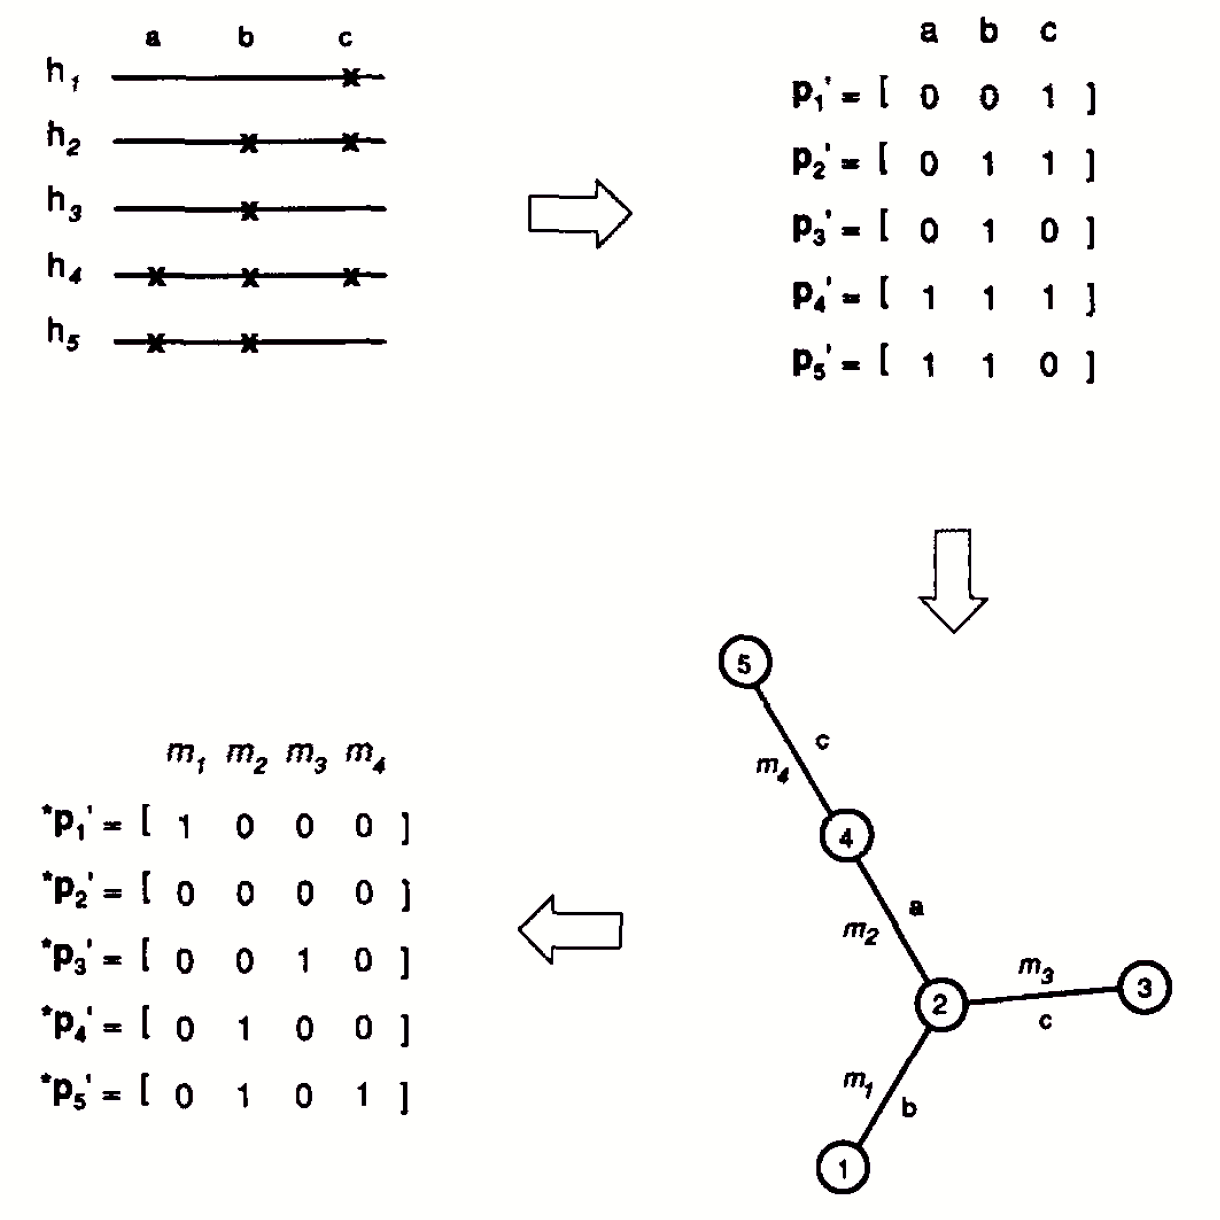
\includegraphics{amova-procedure.eps}}
\end{center}
}

\myslide{
\begin{center}
\resizebox{!}{0.9\textheight}{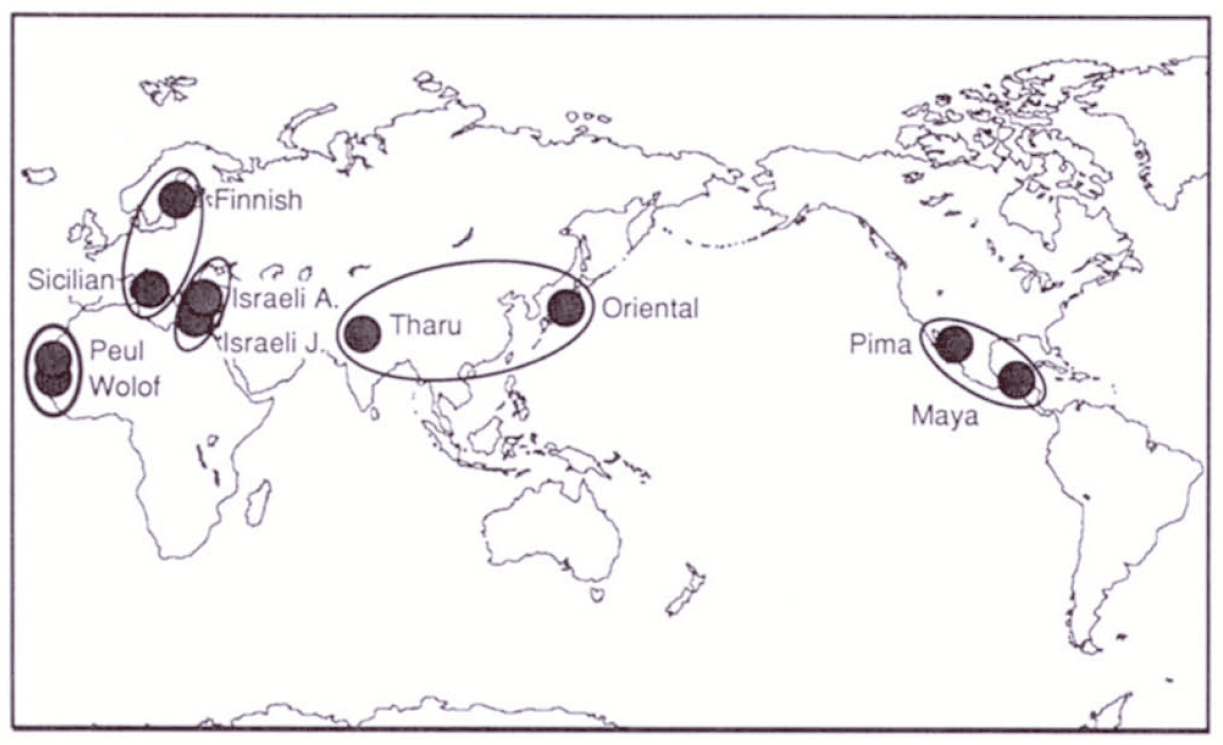
\includegraphics{amova-sample-locations.eps}}
\end{center}
}

\myslide{
\begin{center}
\resizebox{!}{0.9\textheight}{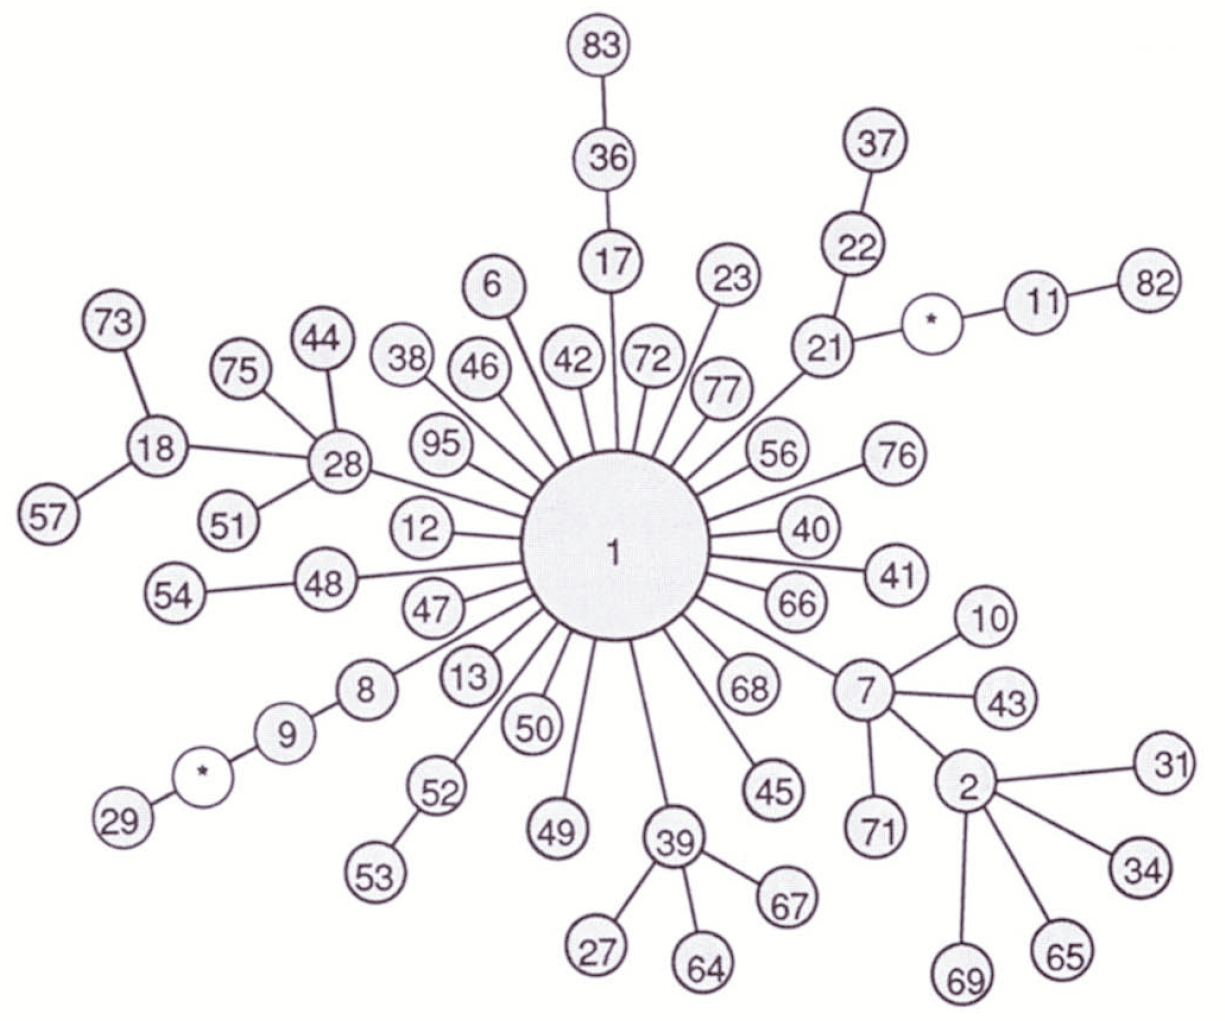
\includegraphics{amova-haplotypes.eps}}
\end{center}
}

\myslide{
\heading{AMOVA results}

\begin{center}
\begin{tabular}{lc}
\hline\hline
Component of differentiation     & $\Phi$-statistics \\
\hline
Among regions                    & $\Phi_{CT} = 0.220$ \\
Among populations within regions & $\Phi_{SC} = 0.044$ \\
Among all populations            & $\Phi_{ST} = 0.246$ \\
\hline
\end{tabular}
\end{center}

\vfill

\begin{eqnarray*}
1 - \Phi_{ST} &=& (1 - \Phi_{SC})(1 - \Phi_{CT}) \\
0.754 &=& (0.956)(0.78)
\end{eqnarray*}

}

\myslide{
\heading{Ancestral polymorphism}

\begin{center}
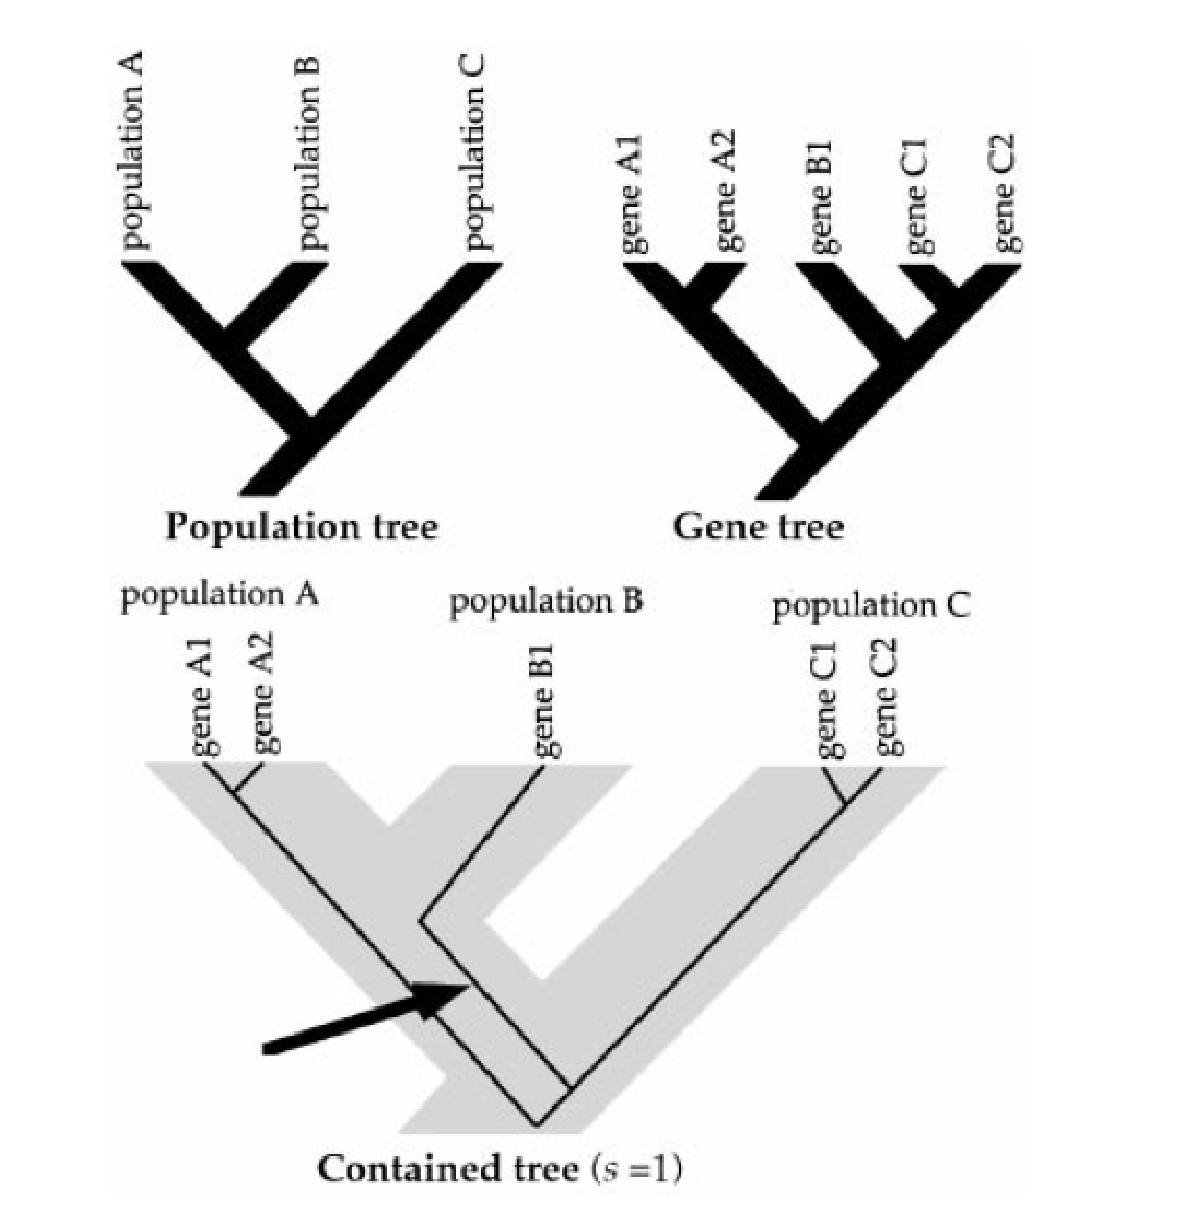
\includegraphics[height=0.9\textheight]{ancestral-polymorphism.eps}
\end{center}

}

\myslide{
\heading{The coalescent in structured populations}

Remember that in a single population
\[
P(t|k, N_e) = \left(\frac{k(k-1)}{4N_e}\right)\left(1-
  \frac{k(k-1)}{4N_e}\right)^{t-1}
\]

\begin{eqnarray*}
P_k(\mbox{coalescent}|n, N_e) &=& \frac{k(k-1)}{4N_e} \\
P(\mbox{no coalescent}|k, N_e, K)
                              &=&\left(1-\frac{k(k-1)}{4N_e}\right)^K \\
P(\mbox{no migration}|k,m, K) &=& (1-m)^{kK}
\end{eqnarray*}
}

\myslide{
\heading{The coalescent in structured populations}


{\scriptsize
\begin{eqnarray*}
P(\mbox{event}|k, m, N_e, K) &=& 1 - P(\mbox{no coalescent}|k, N_e,
K)P(\mbox{no migration}|k,m, K)
\end{eqnarray*}
}

{\small
\[
P(\mbox{event at }t|k, m, N_e, K) = P(\mbox{event}|k, m, N_e,
K)\left(1 - P(\mbox{event}|k, m, N_e, K)\right)^{t-1} 
\]

\[
P(\mbox{data}|m, N_e) \propto f(n, m, N_e, K)
\]

}

}

\end{document}

